\documentclass[preprint,12pt,authoryear]{elsarticle}
\usepackage{amsmath,amssymb,amsthm,booktabs,array,graphicx,float,placeins,setspace,tabularx}
\usepackage[T1]{fontenc}
\usepackage[utf8]{inputenc}
\usepackage{lmodern,microtype}
\usepackage{xurl}
\usepackage[colorlinks=true,citecolor=blue,linkcolor=blue,urlcolor=black]{hyperref}
\journal{}
\setlength{\emergencystretch}{2em}
\setlength{\textfloatsep}{10pt plus 2pt minus 2pt}
\setlength{\floatsep}{9pt plus 2pt minus 2pt}
\setlength{\intextsep}{9pt plus 2pt minus 2pt}
\setlength{\abovecaptionskip}{6pt}
\setlength{\belowcaptionskip}{2pt}
\graphicspath{{figures/}}
\newtheorem{proposition}{Proposition}

% Three distinct note systems: numbered text notes, table notes, and figure notes.
% Main prose stays 12 pt; explanatory notes use conventional 10 pt type.
\newcommand{\TableNote}[1]{%
  \par\vspace{0.65ex}\noindent
  \begin{minipage}{0.97\linewidth}\footnotesize\singlespacing\raggedright
  \textbf{Table notes.}\enspace #1
  \end{minipage}}
\newcommand{\FigureNote}[1]{%
  \par\vspace{0.55ex}\noindent
  \begin{minipage}{0.95\linewidth}\footnotesize\singlespacing\raggedright
  \textbf{Figure notes.}\enspace #1
  \end{minipage}}
\setlength{\footnotesep}{9pt}


\begin{document}
\begin{frontmatter}

\title{News-Based Economic Risk and GDP Forecasting with Constructed Targets:
Denton Benchmarking and Information-Set Evaluation}
\author[caperc]{Emmanuel Akande\corref{cor1}\fnref{orcid1}}
\ead{eakande@capeeconomicconsult.com}
\author[caperc]{Shakir Tewogbade}
\author[cbn]{Temitope J. Laniran}
\author[cbn]{Elijah Akanni}
\author[caperc]{Oyedamola Funmibi Taiwo}
\author[ui]{Honey Adenike Adeleke}
\author[ui]{Kafayat Ajoke Alobaloke}

\cortext[cor1]{Corresponding author: Emmanuel Akande, CAPE Economic Research and Consulting, 11120 Godwit Ln, Charlotte, NC 28278, USA.}
\fntext[orcid1]{ORCID: \url{https://orcid.org/0000-0002-8201-4072}.}
\address[caperc]{CAPE Economic Research and Consulting, 11120 Godwit Ln, Charlotte, NC 28278, USA}
\address[cbn]{Central Bank of Nigeria, Plot 33, Abubakar Tafawa Balewa Way, Central Business District, Abuja, Federal Capital Territory, Nigeria}
\address[ui]{University of Ibadan, Ibadan, Oyo State, Nigeria}


\begin{abstract}
Newspaper reports contain information about economic stress that may reach forecasters before it appears in national accounts. Assessing their predictive value is difficult when the high-frequency GDP target is itself constructed from annual observations: a final monthly series may depend on annual benchmarks unavailable at the historical forecast date. We examine the incremental forecasting contribution of a fixed monthly Growth/Real Economy (GRE) news-risk measure under alternative treatments of the GDP information set. The GRE score combines the prevalence, severity, and prominence of real-economy risk reporting; its construction and country-specific standardization are held constant throughout the comparison. For additive first-difference Denton disaggregation, we derive the interior response of monthly levels to annual benchmark revisions. Off-diagonal weights have an alternating geometric tail with ratio $\mu=(12\sqrt{438}-289)/143\approx-0.264745$; finite-sample endpoints modify the exact relationship. In the African GDP application, the GRE-augmented model's 12-month RMSFE relative to the GDP-only model changes from 0.9961 with retrospective GDP histories to 1.0048 when lagged GDP is reconstructed under an assumed publication calendar and training-label entry is delayed. At one month the corresponding ratio is 0.9964, but the gain is small and sensitive to the benchmark and inference method. Annual GDP values and admitted training labels remain final-vintage, so the exercise does not reproduce a fully historical-vintage forecast. The findings show why the measured forecasting contribution of a news-based indicator depends on the information used to construct its macroeconomic target and regressors.
\end{abstract}

\begin{keyword}
news-based economic risk \sep GDP forecasting \sep temporal disaggregation \sep
Denton benchmarking \sep information sets \sep forecast evaluation
\par\medskip\textit{JEL classification:} C53; C82; E37; O55.
\end{keyword}
\end{frontmatter}
\singlespacing

\section{Introduction}

News reporting provides a continuous record of changing economic conditions, including pressures on output, employment, prices, credit, and financial markets. This information may be useful where official activity measures appear only after considerable delay. Newspaper-based indicators have therefore become part of the empirical literature on economic uncertainty, risk, and macroeconomic forecasting \citep{baker2016,ahir2022,caldara2022,adaemmer2025,seo2025}. Their value, however, cannot be judged solely by whether adding an index lowers the forecast error in a retrospective exercise. The historical information available to the competing models must also be credible.

That requirement is particularly important when the outcome is constructed rather than directly observed at the frequency of the forecast. Monthly GDP is not available as an official series for much of the African panel studied here. We therefore construct a monthly GDP proxy by distributing annual GDP totals with additive first-difference Denton benchmarking. This provides a consistent accounting path, but the path calculated using the full sample need not be one that an analyst could have constructed in an earlier month. An annual total released after the forecast date may affect not only the monthly levels of that year but also levels in neighboring years. If the resulting final-vintage values enter a forecast model as historical GDP regressors, the comparison can reflect information unavailable at the forecast origin.

The economic signal in this paper is the Growth/Real Economy (GRE) measure, a monthly index derived from newspaper coverage. The measure identifies economically relevant articles that discuss real-economy risks and weights their contributions by the severity and prominence of the language used. It is a domain-specific component of a broader news-based economic risk measurement system, not a direct estimate of GDP and not the broad African Economic Risk Index (AERI) or African Risk Score (ARS). Its vocabulary, article scoring, country assignment, and pre-evaluation standardization are fixed before the forecast comparisons. This allows the paper to ask whether the information in GRE adds to the GDP history without changing the news variable when the treatment of GDP information changes.

The paper makes two connected contributions. The first is an empirical measurement and evaluation design that takes a reproducible newspaper-based real-economy risk series as an independent candidate predictor. The article-level rule makes the source of variation in the score explicit: the share of real-economy risk articles, the severity of their language, and their relative prominence in the observed news flow. The second, and principal methodological contribution, is an assessment of that predictor's incremental value when GDP histories and targets are built from lower-frequency benchmarks. The comparison holds the news score, forecasting specifications, forecast targets, and evaluation sample fixed while changing the annual GDP information permitted at each historical forecast origin. These two parts are inseparable in the empirical question: the newspaper measure provides the candidate information, while the information-set design governs whether its measured forecasting contribution is credible.

Figure~\ref{fig:research_framework} records the sequence of measurement and evaluation. It also separates the final constructed monthly GDP series used to score forecasts from the GDP history permitted at an earlier forecast origin. This distinction is not a claim that the study has recovered all historical GDP vintages. The annual totals used here are taken from a final file, and the numerical values of training outcomes also remain final-vintage even when their entry into estimation is delayed.

\begin{figure}[htbp]
\centering
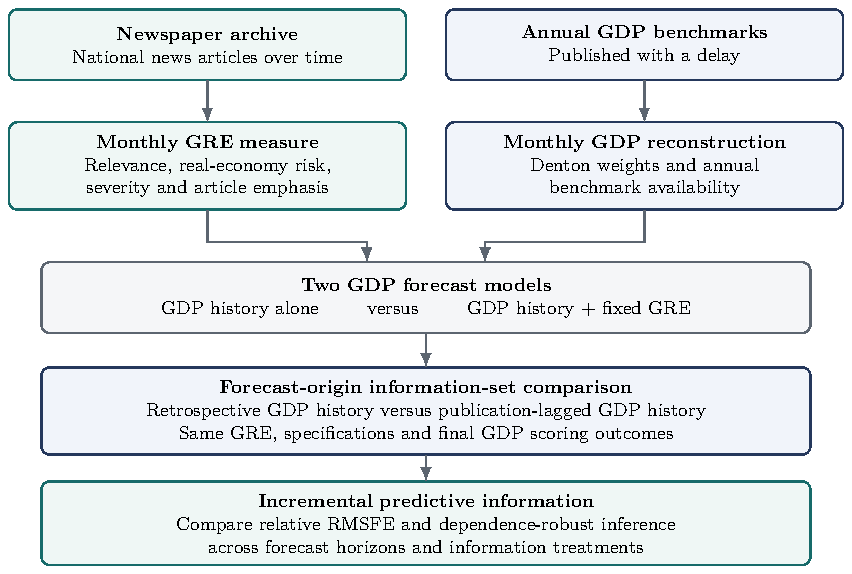
\includegraphics[width=0.98\textwidth]{Figure_Research_Framework.pdf}
\caption{How the news-risk measure and GDP information-set evaluation fit together.}
\label{fig:research_framework}
\FigureNote{The two upper branches have different purposes. Newspaper articles are converted into the fixed monthly GRE predictor; annual GDP totals are used to construct monthly GDP histories. At each forecast origin, annual benchmark eligibility determines the GDP regressors, but both models are ultimately scored against the same final-vintage constructed GDP outcome. The information-set treatment does not alter GRE or establish that historical GDP revisions have been recovered.}
\end{figure}

The analytical question arises from the Denton operator. We show that, away from finite-sample endpoints, the response of a monthly level to annual benchmarks outside its own year follows an alternating geometric tail. For twelve-month annual blocks, successive off-diagonal weights have ratio
\begin{equation}
\mu=\frac{12\sqrt{438}-289}{143}\simeq-0.264745.
\label{eq:intro_mu}
\end{equation}
The magnitude of a coefficient falls by approximately 73.5 percent with each additional annual step, although the first off-diagonal weight depends on the month. This is an exact property of the bounded infinite-block response for additive first-difference Denton. Finite-sample boundary conditions alter the weights, and the result does not determine the sign or size of a change in forecast accuracy. The derivation gives a precise way to establish why a retrospective GDP regressor can depend on later annual benchmarks.\footnote{The 73.5 percent attenuation is a ratio of successive coefficients in the interior geometric tail, not the proportion of GDP or forecast error attributed to an unreleased benchmark. The finite-sample numerical check appears in Supporting Information, Section 1.}

The empirical comparison uses a GDP-only autoregression and the same specification augmented with GRE. Models are estimated recursively at one-, three-, six-, and twelve-month horizons. We compare their performance using full-sample retrospective GDP histories with performance after restricting benchmark-year eligibility and delaying the admission of training labels. At twelve months, GRE relative RMSFE changes from 0.9961 in the retrospective design to 1.0048 under the publication-lagged convention. The one-month relative RMSFE under the latter design is 0.9964, but it is less decisive under two-way dependence-robust inference and a data-rich macroeconomic benchmark. Monte Carlo experiments show that the sign of the information-set distortion is not fixed by the Denton weights.

Our findings concern forecast evaluation using constructed targets, not a universal superiority claim for newspaper-based forecasting. They also leave one important distinction unresolved. Restricting the dates of admissible annual GDP benchmarks does not recover the historical values of previously released GDP, and postponing a final-vintage training label does not make its value historically admissible. We report the resulting exercise as a publication-lagged sensitivity analysis, rather than as a complete historical-vintage backtest.\footnote{The baseline assumes that calendar-year GDP becomes usable in May of the following year. This is an evaluation rule, not a verified release history for each of the 54 economies. July and November rules provide sensitivity checks.}

Section~\ref{sec:constructed} establishes the information-set problem and the Denton weight result. Section~\ref{sec:forecastdesign} explains the construction of GRE, the empirical series, and the forecasting design, followed by Monte Carlo evidence. Section~\ref{sec:application} reports the African GDP application and robustness checks. Section~\ref{sec:conclusion} concludes.

\section{Benchmark Propagation and Information-Set Admissibility}\label{sec:constructed}

\subsection{Constructed monthly values and the forecast-origin information set}

Let $Y_y$ be an annual benchmark and $G_{y,r}$ its constructed monthly level, with $r=1,\ldots,12$. Additive first-difference Denton without an indicator solves\footnote{\emph{Additive} Denton preserves an annual flow total through the sum of its constituent monthly levels. The calculation here uses no auxiliary monthly indicator and penalizes squared changes in adjacent monthly levels. An indicator-assisted or proportional Denton procedure has a different mapping and need not have the root derived below.}
\begin{equation}
\min_{G}\sum_{t=2}^{T}(G_t-G_{t-1})^2
\quad\text{subject to}\quad
\sum_{r=1}^{12}G_{y,r}=Y_y\quad\text{for each year }y.
\label{eq:denton}
\end{equation}
For a fixed set of annual blocks this is a linear map $G=HY$, where $H$ depends on the constraint matrix, the roughness penalty, and sample endpoints. In the empirical illustration the scoring variable is twelve-month log growth constructed from the final path,
\begin{equation}
y^F_{c,t}=100\bigl[\log G^F_{c,t}-\log G^F_{c,t-12}\bigr].
\label{eq:gdp12}
\end{equation}
The superscript $F$ identifies the final-vintage construction used for subsequent scoring; it does not claim that this series existed at earlier forecast origins.\footnote{``Final-vintage'' refers to the frozen final-sample constructed series, not an observed monthly GDP release. The annual series is labeled GDP (PPP)-WEO in the authors' input, but the source file does not provide the IMF release-vintage identifier (Supporting Information, Section 2).}

For a forecast issued at origin $s$, partition the benchmarks into $Y^A_s$, the years permitted by the historical release rule, and $Y^U_s$, those not yet permitted. Partition the Denton operator accordingly. For historical rows required by the forecast, a direct use of the retrospective path contains unavailable-benchmark dependence whenever
\begin{equation}
G^F_{\mathcal H_s}=H_{\mathcal H_s,A}Y^A_s+H_{\mathcal H_s,U}Y^U_s,
\qquad H_{\mathcal H_s,U}\ne 0,
\label{eq:information_condition}
\end{equation}
where $\mathcal H_s$ indexes the months used as regressors. Unless the unavailable benchmarks are already determined by the origin's information set, these rows cannot be reconstructed from information held at $s$. A structural zero in $H_{\mathcal H_s,U}$ removes this particular dependence, but does not itself address revisions to benchmarks counted as released. Re-estimating the monthly path with the admissible annual blocks is an operational remedy for the former problem.

\subsection{Denton weight decay: analytical result}

The following proposition identifies why the dependence extends beyond the benchmarked year. Because a finite constrained smoother has endpoint effects, we state the exact result for the interior impulse-response operator and separately check the finite-sample counterpart.

\begin{proposition}[Alternating geometric tail of annual-benchmark weights]\label{prop:denton}
Consider equation~\eqref{eq:denton} with twelve months per annual block and its bounded impulse response on a doubly infinite sequence of annual blocks. Let $H_{(y_0,r),y}$ be the coefficient of annual total $Y_y$ in month $r$ of year $y_0$. For each $r\in\{1,\ldots,12\}$, constants $C_r^+$ and $C_r^-$ exist such that
\begin{equation}
H_{(y_0,r),y_0+k}=C_r^+\mu^{k-1},\qquad
H_{(y_0,r),y_0-k}=C_r^-\mu^{k-1},\qquad k\geq1,
\label{eq:denton_tail}
\end{equation}
where
\begin{equation}
\mu=\frac{12\sqrt{438}-289}{143}=-0.2647454934\ldots\ .
\label{eq:denton_mu}
\end{equation}
Thus each additional annual step in either off-diagonal tail changes the sign of the monthly-level coefficient and multiplies its absolute value by $|\mu|$. The first off-diagonal coefficients $C_r^+$ and $C_r^-$ depend on the month and need not be fixed fractions of the same-year weight.
\end{proposition}

\begin{proof}
Write $e_y=G_{y,12}$ for the level at the end of year $y$. In an annual block, let $p=e_{y-1}$, $q=e_y$, and let $d_r=G_{y,r}-G_{y,r-1}$ be monthly changes, with $G_{y,0}=p$. Holding $p$, $q$, and $Y_y$ fixed, the within-block minimization is a minimum-norm problem subject to $\sum_{r=1}^{12}d_r=q-p$ and $\sum_{r=1}^{12}(13-r)d_r=Y_y-12p$. Solving its two-constraint normal equations yields the minimized block penalty
\begin{equation}
R(p,q,Y)=\frac{Y^2}{143}-\frac{Yp}{13}-\frac{Yq}{11}
+\frac{23p^2}{78}+\frac{pq}{3}+\frac{25q^2}{66}.
\label{eq:block_penalty}
\end{equation}
The interior first-order condition for $e_y$ in $\sum_j R(e_{j-1},e_j,Y_j)$ is
\begin{equation}
\frac13e_{y-1}+\frac{578}{429}e_y+\frac13e_{y+1}
=\frac{Y_y}{11}+\frac{Y_{y+1}}{13}.
\label{eq:boundary_recurrence}
\end{equation}
The homogeneous equation has characteristic polynomial
$z^2+(578/143)z+1$, whose roots are $\mu$ and $\mu^{-1}$. Since $|\mu|<1$, the bounded response to an impulse in any annual benchmark decays as powers of $\mu$ outside the two adjacent boundary equations directly forced by that benchmark. Finally, the constrained within-year solution is
\begin{equation}
\begin{aligned}
G_{y,r}&=a_r e_{y-1}+b_r e_y+c_rY_y,\\
a_r&=\frac{(r-12)(3r-13)}{156},\qquad
b_r=\frac{r(3r-25)}{132},\qquad c_r=\frac{r(12-r)}{286}.
\end{aligned}
\label{eq:monthly_backsub}
\end{equation}
For a benchmark outside year $y$, the direct term $c_rY_y$ vanishes in its derivative and both boundary responses share the appropriate geometric tail. This proves equation~\eqref{eq:denton_tail}. The supplemental derivation gives the intermediate normal equations and the month-by-month coefficients.\footnote{The characteristic roots are reciprocal because the coefficients on $e_{y-1}$ and $e_{y+1}$ match. Boundedness on a doubly infinite sequence removes the explosive root. A finite panel also satisfies endpoint equations; it should not be treated as though the infinite-lattice formula held exactly throughout.}
\end{proof}

\begin{table}[htbp]
\centering
\caption{Interior geometric attenuation of Denton off-diagonal benchmark weights}
\label{tab:denton_decay}
\begin{tabular}{cr}
\toprule
Additional annual distance $j$ & $|\mu|^j$ \\
\midrule
1 & 0.2647 \\
2 & 0.0701 \\
3 & 0.0186 \\
4 & 0.0049 \\
5 & 0.0013 \\
6 & 0.0003 \\
\bottomrule
\end{tabular}

\TableNote{The figures show the magnitude of the factor multiplying a given off-diagonal coefficient after successive annual steps; they are not GDP shares or estimated leakage rates. The ratio between successive tail coefficients is constant only in the bounded infinite-block solution. The first next-year coefficient depends on the calendar month, and finite-sample endpoints alter the exact weights. The month-specific exposure and finite-sample cross-checks are reported in Supporting Information, Section 1.}
\end{table}


The root is a property of the linear map from annual totals to monthly \emph{levels}; it is not a universal weight on twelve-month growth, which is a nonlinear transformation, and it says nothing by itself about the sign of a difference in forecast loss. For a finite sample, the two endpoint conditions introduce a second homogeneous component. Consequently equation~\eqref{eq:denton_tail} is not an exact finite-panel identity. Direct inversion of the 2015--2025 Denton system confirms rapid convergence toward the interior ratio away from the endpoints; the reproducible comparison is in the supplement. This distinction is essential when a shock is near the beginning or end of an observed panel.\footnote{For the 2015--2025 monthly operator, the supplemental numerical cross-check reports discrepancies of roughly $1.1\times10^{-7}$ and $1.6\times10^{-6}$ for two interior successive-tail ratios around a central 2018 block. These are numerical proximity checks, not an exact finite-sample theorem.}

\subsection{Constructing histories at a forecast origin}

Suppose annual GDP for calendar year $y$ is treated as released in May of $y+1$. At monthly origin $s$ the most recent permitted benchmark is
\begin{equation}
a(s)=\begin{cases}
\operatorname{year}(s)-1,&\operatorname{month}(s)\geq5,\\
\operatorname{year}(s)-2,&\operatorname{month}(s)<5.
\end{cases}
\label{eq:availyear}
\end{equation}
We solve Denton's problem using annual totals only through $a(s)$. For months after the last constrained December and up to $s$, we extrapolate from the last monthly level at the log rate
\begin{equation}
r_{c,s}=\frac{\log Y_{c,a(s)}-\log Y_{c,a(s)-1}}{12}.
\label{eq:extraprate}
\end{equation}
The construction supplies the same forecast-origin GDP history to both competing models.\footnote{Months after the latest allowed December are extrapolations based on the last two allowed annual GDP totals. These monthly extrapolations are modeling inputs, not observations of official monthly GDP. They are recomputed separately at each forecast origin.} In January 2020, for instance, this rule admits annual totals only through 2018; the 2019 total becomes admissible in May 2020.

\begin{figure}[htbp]
\centering
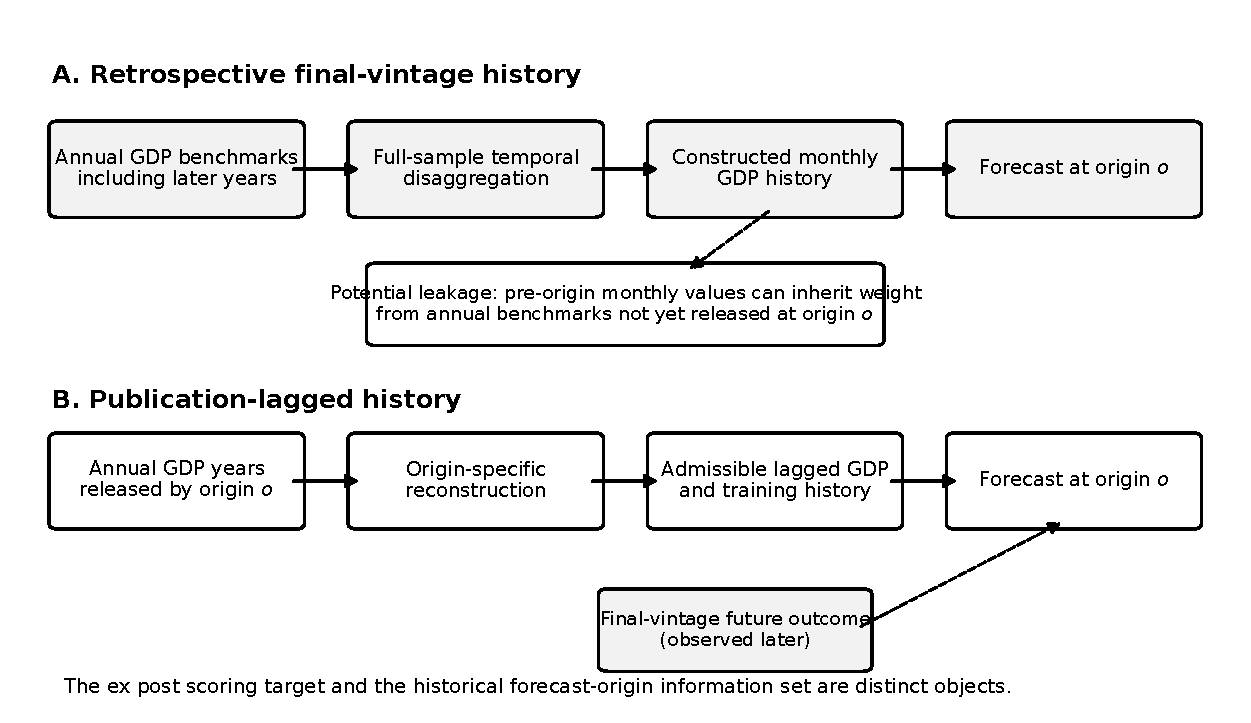
\includegraphics[width=0.96\textwidth]{Figure_Target_Information_Leakage.pdf}
\caption{Retrospective monthly history versus forecast-origin reconstruction.}
\label{fig:leakage}

\FigureNote{Schematic distinction rather than an observed GDP path. The upper history can incorporate annual benchmarks published after the depicted forecast origin. The lower history permits only benchmark years allowed by the assumed calendar and extrapolates unconstrained months; final reconstructed outcomes can still be retained for subsequent scoring. Historical revisions to previously released annual benchmarks are not recovered.}
\end{figure}

The release rule is an assumption, not an archive of actual GDP publication dates. We also consider July and November to assess sensitivity. In recursive estimation the date at which a target may enter is delayed to May of the following year (or the corresponding alternative month). Crucially, the target's \emph{value} remains the final-vintage twelve-month growth constructed from the full annual sample. The delayed-entry rule and reconstructed lags therefore produce an operational publication-lagged comparison, not a fully as-of-date training dataset. A fully historical-vintage design would also reconstruct each previously available training label from its own information set and use the annual values actually released at the time.

\section{News-Based Risk Measurement and Forecast Evaluation}\label{sec:forecastdesign}

\subsection{News coverage and the GRE measurement rule}\label{sec:gre_meas}

The news archive contains 21,303,573 retained article records dated January 2015--December 2025, drawn from an 851-outlet source registry covering 54 African economies. The registry spans English, French, Arabic, and Portuguese-language news outlets, but the frozen GRE activation dictionaries supplied with the replication materials contain explicit English, French, and Portuguese terms; Arabic-only articles may consequently be under-detected. The archive is unbalanced across sources and months, and retained articles are not necessarily distinct news events. Source availability, collection rules, article counts, and duplication checks are documented in Supporting Information, Sections 17--19.\footnote{The 851 outlets form a registry, not a panel of websites successfully scraped in every month. The production archive has 7,127 country-month observations, of which 6,488 have at least 100 retained article records. These figures describe the measurement base; no single article-count threshold defines the forecasting estimand.}

The GRE score summarizes real-economy risk reporting. For each retained article $i$, an economic-relevance indicator $R_i$ identifies whether its normalized text meets a frozen economic dictionary. A second indicator $G_i$ activates the Growth/Real Economy domain, which includes recession, slowdown, contraction, unemployment, and layoffs, with corresponding French and Portuguese terms. Relevant articles receive a severity score $S_i$ on a one-to-four scale, and a bounded weight $W_i$ records headline emphasis, body length, and the presence of multiple economic-risk domains. The monthly country score is
\begin{equation}
\begin{aligned}
GRE_{ct}^{\mathrm{raw}}&=\frac{100}{N_{ct}}\sum_{i\in\mathcal A_{ct}} R_iG_iS_iW_i,\\
W_i&=\min\!\bigl\{2,\max\{1,\,1+0.5T_i+0.2L_i+0.3M_i\}\bigr\}.
\end{aligned}
\label{eq:gre_construction}
\end{equation}
where $N_{ct}$ counts all retained articles in country $c$ and month $t$. Non-qualifying articles remain in the denominator. The score consequently rises when real-economy risk reporting is more prevalent, more severe, or more prominent within the available news coverage. The fixed weighting scheme is a measurement convention; it is not fitted to maximize GDP forecast accuracy. The exact vocabulary, normalization rules, severity tiers, and weighting decisions are recorded in the supplement and replication materials.\footnote{The headline indicator $T_i$ marks a fixed set of risk cues; $L_i$ identifies at least 1,200 normalized body-text characters; $M_i$ identifies two or more active domain dictionaries. Each article contributes once to the domain even if a phrase appears repeatedly. The production indicator measures article records, not unique underlying events.}

\begin{table}[htbp]
\centering\small
\caption{Construction of the Growth/Real Economy news signal}
\label{tab:construction}
\begin{tabularx}{\textwidth}{p{0.19\textwidth}X}
\toprule
Stage & Definition and interpretation \\
\midrule
Economic relevance $R_i$ & Indicator that normalized article text contains economically relevant content. Articles failing this screen contribute zero to the signal but remain in the country-month denominator. \\
Real-economy activation $G_i$ & Indicator that the article activates the frozen Growth/Real Economy dictionary: recession, slowdown, contraction, unemployment, layoffs, and the corresponding French and Portuguese activation terms. Broader GDP/growth vocabulary belongs to the economic-relevance screen rather than this target-specific activation rule. \\
Severity $S_i$ & Ordinal score for relevant articles: 1 = background or mild pressure; 2 = material deterioration; 3 = severe disruption; 4 = extreme or systemic real-economy stress. The highest matched tier applies. \\
Textual emphasis $W_i$ & $\operatorname{clip}(1+0.5T_i+0.2L_i+0.3M_i,1,2)$, where $T_i$ marks headline emphasis, $L_i$ marks at least 1,200 normalized characters, and $M_i$ marks economically dense multi-domain content. \\
Article contribution $Q_i$ & $Q_i=R_iG_iS_iW_i$. Only economically relevant articles that activate the real-economy domain contribute positive weight. \\
Country-month signal $GRE_{ct}$ & $100N_{ct}^{-1}\sum_{i\in\mathcal A_{ct}}Q_i$, where $N_{ct}$ is the total number of retained articles. The signal therefore reflects both the prevalence and the intensity of real-economy risk reporting. \\
\bottomrule
\end{tabularx}
\TableNote{All scores are computed from retained normalized article text with a fixed rule; neither severity tiers nor emphasis coefficients are fitted to GDP outcomes. The denominator includes articles that do not activate the real-economy domain, so a zero contribution does not imply exclusion from the archive.}
\end{table}


Before estimation, we standardize the monthly GRE score separately for each country using its 2015--2018 mean and standard deviation. Those calibration statistics are frozen ahead of the January 2020 evaluation start. For the remainder of the paper, $GRE_{ct}$ denotes this standardized score. Its construction, including the country assignment, is unchanged across the retrospective and publication-lagged GDP exercises. Changes in the forecast rankings therefore cannot be attributed to reweighting or reselection of the news predictor.

\begin{figure}[htbp]
\centering
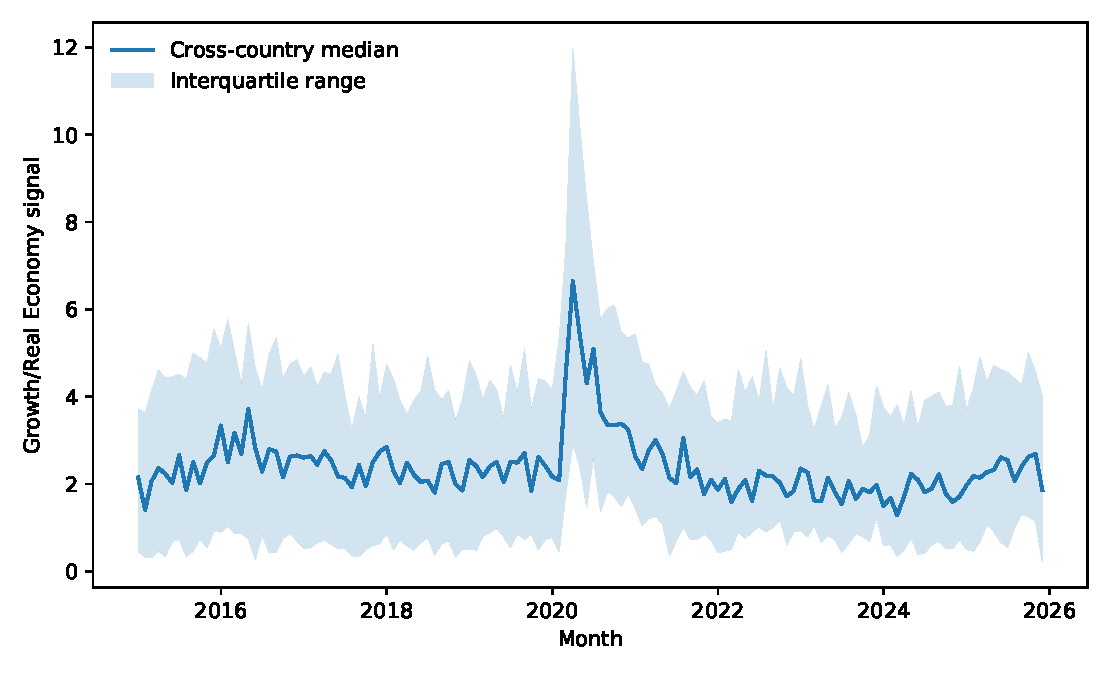
\includegraphics[width=0.79\textwidth]{Figure_0_GRE_Descriptive.pdf}
\caption{Cross-country distribution of the monthly GRE news-risk measure, 2015--2025.}
\label{fig:gre_description}
\FigureNote{The line plots the median GRE score across economies with observed news records in each month; shading indicates the interquartile range. The display describes variation in the measured news signal, not official GDP growth. Coverage changes over time and the country composition need not be balanced. The score in this display precedes the country-specific forecast-model standardization.}
\end{figure}

\subsection{Constructed GDP, sample, and release conventions}

The GDP side of the comparison comprises an author-supplied annual activity series labeled ``GDP (PPP)-WEO'' for 2015--2025. Its workbook does not identify a particular IMF World Economic Outlook release or archive historical annual-data vintages. We therefore refer to the series as final-vintage, WEO-labeled annual benchmarks rather than attribute the values to a verified release. Monthly GDP levels are constructed by equation~\eqref{eq:denton}, and the common outcome is twelve-month growth in that final-vintage monthly series. Forecast targets run from January 2020 through December 2025 in an unbalanced country panel.\footnote{There are 72 target months per forecast horizon, with varying country availability. The separate balanced diagnostic of cross-country dependence uses 53 countries (Supporting Information, Section 11).}

The baseline annual release rule is May of the year following the benchmark year, as in equation~\eqref{eq:availyear}. We repeat the evaluation with July and November conventions. The GDP histories supplied to both forecast models are rebuilt at each origin using annual years permitted under the selected rule. Training targets are admitted only after their assumed release date but retain their final-vintage numerical values. These restrictions address an important source of retrospective information use, but they do not recover subsequent revisions to the annual GDP data or create historically consistent training labels. The evaluation design is summarized in Table~\ref{tab:design}.

\begin{table}[htbp]
\centering\scriptsize\singlespacing
\caption{Publication-lagged final-vintage forecasting design}
\label{tab:design}
\renewcommand{\arraystretch}{0.92}
\begin{tabularx}{\textwidth}{p{0.24\textwidth}X}
\toprule
Element & Implementation \\
\midrule
Country universe & Fifty-four African economies; membership is determined by pre-evaluation data availability only. \\
Annual GDP source & Author-supplied annual series labeled ``GDP (PPP)-WEO,'' 2015--2025. The replication copy is frozen as supplied on 13 September 2026. The workbook does not identify the underlying WEO publication vintage, so the annual values are treated as final-vintage data rather than historical real-time vintages. \\
Realized evaluation target & Twelve-month growth of a final-vintage monthly GDP-PPP proxy constructed by additive first-difference Denton and constrained to aggregate exactly to the annual benchmarks. This series scores realized outcomes and supplies the final-vintage labels of training observations admitted by the release-date rule. \\
Forecast-origin GDP information & At each forecast origin, lagged monthly GDP growth is reconstructed from annual benchmark years permitted by the release rule. Under the baseline rule, year $y$ becomes usable from May of $y+1$. Denton is applied only through the last permitted annual year; subsequent months up to the forecast origin are extrapolated using the log-monthly rate implied by the two most recent permitted annual totals. \\
Training-target availability & A target dated in year $y$ enters estimation only from May of $y+1$. Its value is nevertheless the final-vintage Denton outcome, so this restriction does not create fully historical training labels. \\
Text scaling & Country-specific GRE and comparator means and standard deviations are estimated over 2015--2018 and frozen before the January 2020 evaluation start. \\
Benchmark & Pooled country-fixed-effects autoregression using three publication-lagged GDP-growth lags and target-month seasonal indicators. GRE adds one standardized news regressor at the forecast origin. \\
Evaluation & Recursive target dates January 2020--December 2025 at 1-, 3-, 6-, and 12-month forecast horizons. The full horizon profile is reported; no new horizon is relabeled as pre-specified after inspection of the corrected results. \\
Release-timing sensitivity & Baseline May availability is repeated using July and November release conventions. \\
Inference & RMSFE, MAE, target-month HAC Clark--West inference, complementary two-way country--target-month covariance, Holm correction across horizons, cross-section-preserving moving-block bootstrap, and country-level RMSFE ratios. \\
\bottomrule
\end{tabularx}
\TableNote{Annual GDP values are taken from the author-supplied workbook frozen on 13 September 2026 and identified there as ``GDP (PPP)-WEO''; the precise WEO release is not recorded. The May release month is a common modeling convention, not an observed date for each economy. Admitted training outcomes still use the final-vintage Denton values. Consequently, ``publication-lagged'' refers to benchmark-year eligibility and target-entry dates, not complete historical-vintage consistency (Supporting Information, Section 2).}
\end{table}


\subsection{Benchmark and GRE-augmented models}

The forecast comparison uses the same country panel, target dates, horizons, seasonal controls, and estimation scheme under both information treatments. The benchmark contains only GDP history and fixed effects. For horizon $h$,
\begin{equation}
M_0:\qquad
y^F_{c,t+h}=\alpha_c+\sum_{j=0}^{2}\phi_{j,h}y^{I(t)}_{c,t-j}
+\sum_{m=2}^{12}\delta_{m,h}\mathbf{1}\{M_{t+h}=m\}+u_{c,t+h},
\label{eq:benchmark}
\end{equation}
where $y^{I(t)}_{c,t-j}$ is twelve-month GDP growth reconstructed from the information allowed at forecast origin $t$, $\alpha_c$ is a country fixed effect, and the target-month indicators allow for seasonal differences in forecast outcomes.

The augmented model adds one variable, standardized GRE measured at the forecast origin:
\begin{equation}
\begin{aligned}
M_1:\quad y^F_{c,t+h} &= \alpha_c+\sum_{j=0}^{2}\phi_{j,h}y^{I(t)}_{c,t-j}+\beta_h GRE_{c,t}\\
&\quad +\sum_{m=2}^{12}\delta_{m,h}\mathbf{1}\{M_{t+h}=m\}+v_{c,t+h}.
\end{aligned}
\label{eq:augmented}
\end{equation}
Separate coefficients are estimated for each forecast horizon. $M_0$ uses the specified GDP history alone; $M_1$ adds the contemporaneous GRE score to that history. The news variable, country set, and model form do not change between the retrospective and publication-lagged exercises.

\subsection{Recursive forecasting procedure}

Forecasts are generated one origin at a time. At each origin $t$ we first determine the annual GDP years allowed by the release rule. Those annual observations are used to rebuild the monthly GDP history through the last permitted benchmark and to extrapolate the remaining months up to $t$. We then determine which past target dates have passed the assumed annual release threshold for entry into the estimation sample. The admitted target values remain final-vintage constructions, not values reconstructed from historical annual vintages.\footnote{A release-date restriction governs when a target may enter training. It does not make the target's numerical value vintage-consistent: final Denton weights can depend on future annual blocks even for a target whose calendar year has already been released.} Both models are estimated on that expanding sample, forecasts are produced for $t+h$, and the origin moves forward by one month. After the target date has passed, both forecasts are scored against the same final-vintage monthly GDP outcome.

At each forecast origin we:
\begin{enumerate}
\item identify the annual GDP benchmarks available at origin $t$;
\item reconstruct the monthly GDP history that could be formed from those benchmarks;
\item admit only training dates permitted by the target-release rule, retaining their final-vintage target values;
\item estimate $M_0$ and $M_1$ on the same expanding sample;
\item produce the $h$-month-ahead forecasts; and
\item score both forecasts against the common final-vintage outcome after it is observed.
\end{enumerate}
The procedure is repeated for every target month from January 2020 through December 2025 and for horizons $h=1,3,6,12$.

\subsection{What changes between the two information designs}

The retrospective and publication-lagged designs are not two different forecasting models. They use the same models and the same realized target. They differ in what is treated as historically available. Table~\ref{tab:designcontrast} records that distinction.

\begin{table}[htbp]
\centering\small\singlespacing
\caption{Retrospective and publication-lagged forecast designs}
\label{tab:designcontrast}
\renewcommand{\arraystretch}{1.03}
\begin{tabularx}{\textwidth}{p{0.25\textwidth}XX}
\toprule
Element & Retrospective final-vintage design & Publication-lagged final-vintage design \\\\
\midrule
Final scoring target & Final-vintage monthly GDP path & Same final-vintage monthly GDP path \\\\
Forecast models & $M_0$ and $M_1$ & Same $M_0$ and $M_1$ \\\\
GRE predictor and scaling & Fixed GRE; 2015--2018 scaling & Same GRE and scaling \\\\
Countries and horizons & 54 countries; 1, 3, 6, 12 months & Same countries and horizons \\\\
GDP lags at forecast origin & Taken from the full final-vintage Denton history & Rebuilt from annual benchmarks permitted at the origin \\\\
Training-target entry & Final-vintage targets treated as immediately usable & The same final-vintage targets enter after the assumed release date \\\\
Estimation & Recursive expanding window & Same recursive expanding window \\\\
\bottomrule
\end{tabularx}
\TableNote{Entries describe the information permitted when forecasts are generated; they do not denote two different statistical models. ``Publication-lagged'' restricts forecast-origin GDP benchmarks and the entry date of training outcomes, but uses final-vintage benchmark values and final-vintage training-label values. Both columns are scored against identical constructed GDP growth. Historical annual revisions are not represented.}
\end{table}

Because the models and scoring target are fixed, the 12-month change from 0.9961 to 1.0048 follows from the GDP-lag and training-entry restrictions in these two designs, not from altering the news measure, countries, or scoring outcome. Neither design uses archived annual GDP vintages, and the delayed training labels themselves retain final-sample benchmark dependence.

\subsection{Forecast loss and inference}

For model $j$ and horizon $h$, let $e_{j,c,t+h}$ be the forecast error. We report root mean squared forecast error,
\begin{equation}
RMSFE_j(h)=\left[\frac{1}{N_h}\sum_{c,t} e_{j,c,t+h}^2\right]^{1/2},
\end{equation}
and mean absolute error. The main comparison is the relative RMSFE,
\begin{equation}
\rho_h=\frac{RMSFE_{M_1}(h)}{RMSFE_{M_0}(h)}.
\label{eq:relative_rmsfe}
\end{equation}
Values below one favor the GRE-augmented model; values above one favor the benchmark.\footnote{A relative RMSFE of 0.9964 corresponds to approximately $100(1-0.9964)=0.36$ percent lower RMSFE, not a 0.36-percentage-point reduction in GDP growth. RMSFE and MAE themselves are expressed in percentage points of twelve-month log growth.}

Because $M_0$ is nested in $M_1$, equal-predictive-accuracy tests use the Clark--West adjusted loss differential \citep{clarkwest2007}.\footnote{The Clark--West statistic adjusts the squared-error comparison for the estimation noise introduced by a larger nested model. Its one-sided $p$-value is not a test of the exact unadjusted RMSFE ratio printed in the tables. The paired bootstrap for raw RMSFE addresses a different inferential object.} Forecast errors are correlated across countries and across overlapping target months. The main test averages the adjusted differential across countries within each target month and applies Newey--West HAC inference. We also report two-way covariance clustered by country and target month \citep{qu2024,akgun2024,coroneo2025}, Holm adjustment across the four horizons, and a moving-block bootstrap that resamples target months while preserving the full contemporaneous country cross-section. The one-month balanced diagnostic panel has a mean pairwise forecast-error correlation of about 0.442 and a Pesaran CD statistic of about 139.2, so independent-country inference would be inappropriate.

\subsection{Monte Carlo evidence on forecast-ranking distortions}

The simulation keeps the target-construction problem separate from the details of the African application. Each replication contains 54 economies observed monthly from 2015 through 2025. Annual GDP follows a panel process with country-specific average growth, a common annual component, and idiosyncratic shocks. The same first-difference Denton operator converts annual GDP to monthly frequency. Forecasts use three lags of twelve-month growth and country fixed effects.

We use two signal designs and one placebo. In the current-state design, the alternative variable measures the contemporaneous annual activity innovation with noise and contains no next-year innovation. The persistent-state stress design raises annual persistence and the signal-to-noise ratio so that the retrospective 12-month comparison can reverse in the same direction as the empirical application. Its parameters are not estimated from the African panel. The placebo replaces the signal with independent noise. Each design is run under the full final-vintage Denton history and under the publication-lagged rule.

\begin{table}[htbp]
\centering
\small
\caption{Monte Carlo: target-information treatment and the horizon profile of text value}
\label{tab:simulation}
\resizebox{\textwidth}{!}{%
\begin{tabular}{@{}llrrr@{}}
\toprule
DGP & Design & $h$ & Mean relative RMSFE & Share with RMSFE gain \\
\midrule
Current-state signal & Retrospective final-vintage & 1 & 1.0002 & 39.0\% \\
Current-state signal & Publication-lagged & 1 & 0.9969 & 97.7\% \\
Current-state signal & Retrospective final-vintage & 3 & 1.0002 & 36.6\% \\
Current-state signal & Publication-lagged & 3 & 0.9973 & 96.5\% \\
Current-state signal & Retrospective final-vintage & 6 & 1.0002 & 39.2\% \\
Current-state signal & Publication-lagged & 6 & 0.9987 & 84.6\% \\
Current-state signal & Retrospective final-vintage & 12 & 1.0001 & 47.5\% \\
Current-state signal & Publication-lagged & 12 & 1.0025 & 47.6\% \\
\midrule
Persistent-state stress & Retrospective final-vintage & 12 & 0.9962 & 90.2\% \\
Persistent-state stress & Publication-lagged & 12 & 1.0122 & 35.1\% \\
\bottomrule
\end{tabular}}

\TableNote{Entries are the mean of the augmented-model RMSFE divided by benchmark RMSFE over 1,000 independently generated panels; ``share with gain'' is the fraction of replications for which that ratio is below one. The simulation represents 54 countries over the 2015--2025 calendar. The persistent-state specification deliberately raises annual persistence from 0.25 to 0.95 and increases signal-to-noise; it is an existence test, not an estimated model of the African data. Additional designs and the pure-noise placebo are in Supporting Information, Section 3.}
\end{table}


\begin{figure}[htbp]
\centering
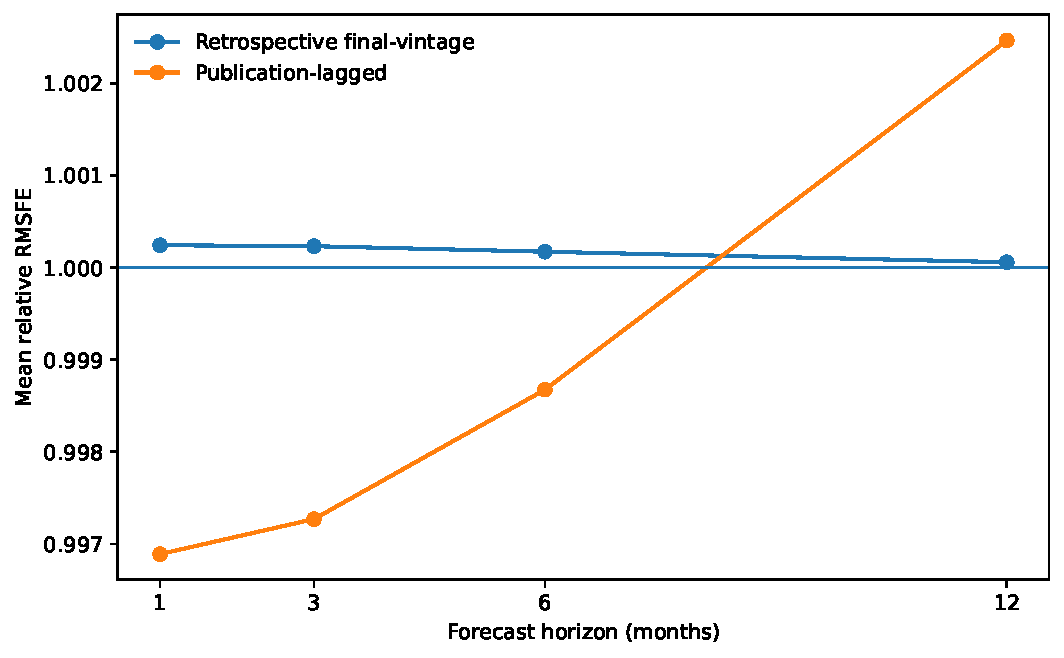
\includegraphics[width=0.76\textwidth]{Figure_Simulation_Horizon_Distortion.pdf}
\caption{Monte Carlo horizon profile under retrospective and publication-lagged target information.}
\label{fig:simulation}

\FigureNote{Each point is the mean relative RMSFE over 1,000 replications for the current-state signal design (54 economies, 2015--2025). Values below one favor the augmented model. The news-like signal contains the current annual innovation with noise, not the next-year innovation. The persistent-state stress design and independent-noise placebo are reported separately in Supporting Information; the chart does not summarize them.}
\end{figure}

The two signal designs give different answers. In the current-state design, the one-month relative RMSFE is 1.0002 with retrospective information and 0.9969 with publication-lagged information. At twelve months both ratios are close to one. In the persistent-state stress design, the 12-month ratio is 0.9962 under the retrospective history and 1.0122 under publication timing. The placebo stays near one. The information error can hide a short-horizon gain or create a long-horizon gain. Its sign is not fixed by the Denton operator.


\section{Empirical Evidence from African GDP}\label{sec:application}

\subsection{The 12-month ranking reversal}

The retrospective design used the final-vintage Denton series twice: as the realized outcome and as lagged GDP information. Under that treatment, the 12-month relative RMSFE is 0.9961. Rebuilding lagged GDP histories at each forecast origin and delaying training outcomes until the assumed release date raises the ratio to 1.0048. The ranking switches sides of unity, although both deviations from one are small.

\begin{table}[htbp]
\centering\small\singlespacing
\caption{Target-information audit: final-vintage lags versus publication-lagged lags}
\label{tab:target_audit}
\begin{tabularx}{\textwidth}{p{0.35\textwidth}rrX}
\toprule
Design & Horizon & Relative RMSFE & Interpretation \\
\midrule
Final-vintage monthly GDP treated as available at origin & 12 & 0.9961 & Retrospective diagnostic only; nominal CW $p=0.033$. \\
Publication-lagged GDP information set & 12 & 1.0048 & No long-horizon GRE gain; HAC CW $p=0.905$. \\
Publication-lagged GDP information set & 1 & 0.9964 & Modest short-horizon predictive content; HAC CW $p=0.0006$. \\
\bottomrule
\end{tabularx}
\vspace{0.35em}

\TableNote{The retrospective line is an audit of a specification that used the final GDP reconstruction as both a scoring outcome and a historical predictor. It is not interpreted as a feasible forecast backtest. All rows keep the same final-vintage scoring outcomes. The May-rule design reconstructs forecast-origin GDP lags and delays training-label entry, but does not reconstruct the labels from archived vintages. Clark--West $p$-values test an adjusted nested-model loss differential, not the reported raw RMSFE ratio itself.}
\end{table}


The correction affects both forecast-origin GDP lags and the date at which realized targets enter recursive estimation. We separate those channels with four designs. $R$ is the original retrospective design, $L$ corrects only lagged GDP, $T$ corrects only training-outcome timing, and $P$ applies both. If $\rho_d$ is GRE RMSFE divided by benchmark RMSFE under design $d$, the total change is
\[
\Delta_{P-R}=\rho_P-\rho_R.
\]
We allocate it with a two-factor Shapley calculation,
\[
\phi_{\mathrm{lag}}=\tfrac12[(\rho_L-\rho_R)+(\rho_P-\rho_T)],\qquad
\phi_{\mathrm{train}}=\tfrac12[(\rho_T-\rho_R)+(\rho_P-\rho_L)].
\]
A 5,000-draw circular moving-block bootstrap resamples 12 consecutive target months and keeps all countries together within each selected month.

\begin{table}[htbp]
\centering\small
\caption{Formal decomposition of the 12-month target-information correction}
\label{tab:channel_decomposition}
\begin{tabularx}{\textwidth}{@{}>{\raggedright\arraybackslash}Xcc@{}}
\toprule
\multicolumn{3}{l}{\textit{Panel A. Nested information-set designs}} \\
Design & Relative RMSFE & Relative MAE \\
\midrule
Retrospective: final-vintage lags + immediate training & 0.9961 & 0.9930 \\
GDP-lag corrected only & 1.0017 & 1.0070 \\
Training-timing corrected only & 0.9966 & 0.9967 \\
Fully publication-lagged & 1.0048 & 1.0122 \\
\midrule
\multicolumn{3}{l}{\textit{Panel B. Paired 12-month block-bootstrap decomposition of relative RMSFE}} \\
Contrast & Change in relative RMSFE & 95\% bootstrap interval \\
\midrule
Total correction, $P-R$ & +0.0088 & [+0.0048, +0.0171] \\
GDP-lag channel, Shapley contribution & +0.0069 & [+0.0042, +0.0145] \\
Training-timing channel, Shapley contribution & +0.0018 & [-0.0018, +0.0075] \\
\bottomrule
\end{tabularx}

\TableNote{For the two binary restrictions, $R$ denotes neither restriction, $L$ lag-history restriction only, $T$ training-entry restriction only, and $P$ both. Panel B averages the two possible orders in which restrictions can be imposed, allocating the nonlinear change in relative RMSFE. Intervals come from 5,000 circular moving-block draws of 12 consecutive target months, with the cross-section kept intact. This is a descriptive allocation between evaluation designs, not a causal share of Denton leakage. Direct tests of paired raw and Clark--West loss differences are supplied in Supporting Information.}
\end{table}


At twelve months, correcting only the lagged GDP history moves the ratio from 0.9961 to 1.0017. Correcting only training timing gives 0.9966. Applying both corrections gives 1.0048. The total change is $+0.0088$, with a paired block-bootstrap 95 percent interval of $[0.0048,0.0171]$. The lag-history contribution is $+0.0069$ with interval $[0.0042,0.0145]$, about 79 percent of the total. The training contribution is $+0.0018$ and its interval includes zero. Within this pair of operational designs, most of the reversal is associated with replacing retrospective GDP regressors. The decomposition is descriptive and should not be read as a structural causal attribution.\footnote{For two restrictions, the Shapley contribution averages the marginal change from introducing a restriction first and from introducing it second. The shares depend on the specified four designs and aggregate relative-RMSFE functional; they do not identify an exogenous treatment effect or partition a physically observed quantity of leaked information.}

Figure~\ref{fig:empirical_reversal} shows the result across horizons.

\begin{figure}[htbp]
\centering
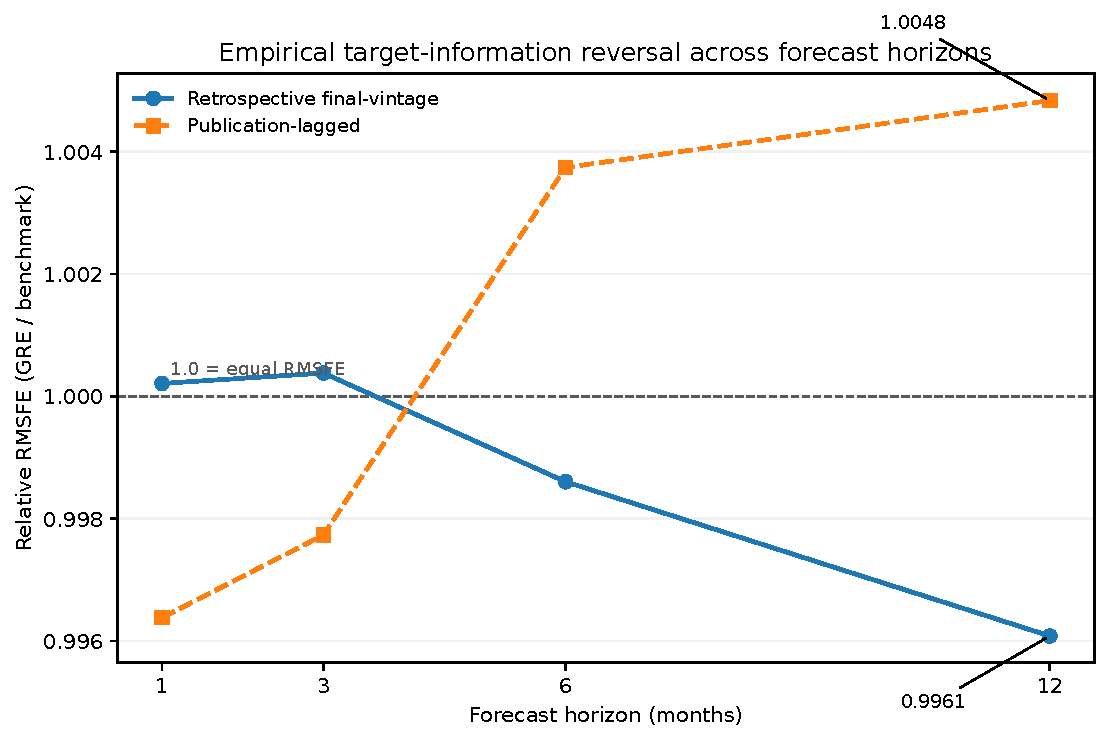
\includegraphics[width=0.82\textwidth]{Figure_Empirical_Horizon_Reversal.pdf}
\caption{Empirical horizon profile under retrospective final-vintage and publication-lagged information.}
\label{fig:empirical_reversal}

\FigureNote{Forecast models, GRE observations, country set, and final scoring targets are held fixed between designs. The retrospective design uses final-sample GDP histories as regressors; the publication-lagged design restricts annual benchmark-year eligibility and the entry date of final-vintage training labels. The common May release convention is assumed rather than verified country by country. Vertical differences describe sensitivity to the treatment of GDP information, not a causal effect of GRE.}
\end{figure}

\subsection{The reversal is not a pandemic result}

The same comparison is repeated after removing all 2020--2021 forecast targets. The retrospective 12-month ratio remains below one at 0.9976, while the publication-lagged ratio rises to 1.0133. Removing the pandemic period does not explain the reversal; it makes the difference larger.\footnote{Only target months in 2020--2021 are excluded from evaluation. Earlier observations remain in the recursive training history when allowed by the information rule; this is not a refitting exercise that discards all pandemic-era observations from model estimation.}

\begin{table}[htbp]
\centering
\caption{Forecast robustness excluding the 2020--2021 pandemic period}
\label{tab:excovid}
\begin{tabular}{llcccc}
\toprule
Sample & Information design & $h=1$ & $h=3$ & $h=6$ & $h=12$ \\
\midrule
2020--2025 & Retrospective & 1.0002 & 1.0004 & 0.9986 & 0.9961 \\
2020--2025 & Publication-lagged & 0.9964 & 0.9977 & 1.0037 & 1.0048 \\
2022--2025 & Retrospective & 1.0001 & 1.0002 & 0.9995 & 0.9976 \\
2022--2025 & Publication-lagged & 0.9926 & 0.9929 & 0.9988 & 1.0133 \\
\midrule
\multicolumn{6}{l}{\textit{Publication-lagged 2022--2025 inference}} \\
Horizon & Relative MAE & \multicolumn{2}{c}{CW HAC $p$} & \multicolumn{2}{c}{CW two-way $p$} \\
\midrule
1 month & 0.9863 & \multicolumn{2}{c}{$<0.001$} & \multicolumn{2}{c}{0.0271} \\
3 months & 0.9887 & \multicolumn{2}{c}{0.0014} & \multicolumn{2}{c}{0.0289} \\
6 months & 0.9978 & \multicolumn{2}{c}{0.0811} & \multicolumn{2}{c}{0.1583} \\
12 months & 1.0229 & \multicolumn{2}{c}{0.9697} & \multicolumn{2}{c}{0.7706} \\
\bottomrule
\end{tabular}

\TableNote{Each horizon entry in the first panel is GRE RMSFE divided by the benchmark RMSFE; a value below one favors GRE. The restriction drops target months in January 2020--December 2021 from scoring, but leaves the recursive estimation history and the publication rule unchanged. The lower panel contains one-sided Clark--West $p$-values; the target-month HAC and country-by-target-month two-way procedures address different dependence assumptions.}
\end{table}


The release month is also uncertain across 54 economies. Repeating the reconstruction with July and November availability leaves the one-month point estimates close to the May result. At one month, relative RMSFE is 0.9964 under May, 0.9969 under July, and 0.9973 under November. The 12-month conclusion remains unfavorable under the corrected design. The release-calendar exercise is a timing sensitivity check, not a claim that every country publishes annual GDP on the same date.

\begin{table}[htbp]
\centering\small
\caption{Sensitivity of the one-month GRE result to annual-data release timing}
\label{tab:release_timing}
\resizebox{\textwidth}{!}{%
\begin{tabular}{lrrrrrr}
\toprule
Annual year $y$ usable from & Rel. RMSFE & Rel. MAE & HAC CW $p$ & Two-way $p$ & Bootstrap CW $p$ & Countries $<1$ \\
\midrule
May of $y+1$ & 0.9964 & 0.9897 & 0.0006 & 0.053 & 0.037 & 33/54 \\
July of $y+1$ & 0.9969 & 0.9894 & 0.0004 & 0.039 & 0.038 & 31/54 \\
November of $y+1$ & 0.9973 & 0.9910 & 0.0001 & 0.030 & 0.019 & 32/54 \\
\bottomrule
\end{tabular}}
\vspace{0.35em}

\TableNote{Annual totals for year $y$ are treated as eligible starting in the listed month of $y+1$, with no claim that all countries used that calendar. The denominator of ``Countries $<1$'' is 54; the numerator counts countries whose one-month GRE RMSFE is below their own benchmark RMSFE. The 5,000-draw bootstrap resamples 12-month target-date blocks across the full country cross-section. See the supplement for the separate age-of-information and revision diagnostics; neither establishes a mechanism.}
\end{table}


\subsection{What remains at short horizons}

Under the baseline publication rule, the one-month benchmark RMSFE is 8.375 and the GRE RMSFE is 8.344, giving relative RMSFE 0.9964. Relative MAE is 0.9897. At three months the RMSFE ratio is 0.9977; at six months it is 1.0037; at twelve months it is 1.0048.

\begin{table}[htbp]
\centering\scriptsize
\caption{Publication-lagged forecast performance of the GRE-augmented model}
\label{tab:main_results}
\resizebox{\textwidth}{!}{%
\begin{tabular}{rrrrrrrr}
\toprule
$h$ & Benchmark RMSFE & GRE RMSFE & Rel. RMSFE & Benchmark MAE & GRE MAE & HAC CW $p$ & Two-way $p$ \\
\midrule
1  & 8.375 & 8.344 & 0.9964 & 5.441 & 5.385 & 0.0006 & 0.053 \\
3  & 8.493 & 8.473 & 0.9977 & 5.523 & 5.483 & 0.041 & 0.084 \\
6  & 8.588 & 8.620 & 1.0037 & 5.513 & 5.529 & 0.878 & 0.869 \\
12 & 19.264 & 19.357 & 1.0048 & 7.028 & 7.114 & 0.905 & 0.872 \\
\bottomrule
\end{tabular}}
\vspace{0.35em}

\TableNote{Errors are measured against final-vintage twelve-month log GDP growth, expressed in percentage points. Relative RMSFE is GRE RMSFE divided by benchmark RMSFE; the relative MAE ratios are 0.9897, 0.9928, 1.0028, and 1.0122 at horizons 1, 3, 6, and 12 months. The baseline assumes each annual benchmark becomes usable in May of the following year. Clark--West values are one-sided adjusted-loss tests. Holm correction across four horizons yields HAC-adjusted $p=0.0023$ at one month and $p=0.122$ at three months; corresponding two-way adjusted values are 0.211 and 0.253. A bootstrap interval for the raw one-month RMSFE improvement includes zero (Supporting Information, Sections 4--6).}
\end{table}


The one-month Clark--West result is strong under target-month HAC inference ($p=0.0006$) and weaker under two-way clustering ($p=0.053$). A 5,000-draw moving-block bootstrap gives a one-sided Clark--West value of 0.037, but the 95 percent interval for the raw percentage RMSFE improvement is approximately $[-0.50,1.44]$.\footnote{The apparently different messages are not contradictory. The Clark--West resampling result concerns mean adjusted loss, while the interval measures improvement in the raw ratio of root-mean-squared errors. The latter includes zero improvement, so the size and even the sign of the unadjusted gain remain uncertain.} Country results are mixed: 33 of 54 economies have lower one-month RMSFE with GRE and 21 do not. After removing 2020--2021, the one-month ratio improves to 0.9926.

The online supplement reports three checks on this short-horizon result. Exact-text deduplication changes the one-month ratio only from 0.9964 to 0.9969. Splitting forecast origins by the age of the annual information set gives suggestive results under the May and July conventions but not under November, and a direct regression of loss improvement on information age is weak. GRE also does not significantly predict the revision from the publication-lagged current-growth estimate to final-vintage growth. We do not assign a causal mechanism to the one-month result.

\subsection{A richer conventional benchmark}

We next replace the parsimonious benchmark with a panel of up to 162 monthly macroeconomic series: publication-lagged GDP growth, inflation, and exchange-rate depreciation for each economy. After removing series with limited pre-evaluation coverage or negligible variance, 159 remain. Means, standard deviations, and principal-component loadings are estimated only on March 2016--December 2018 and then frozen. Six factors explain 82.1 percent of calibration-sample variance.\footnote{The choice of six factors uses only the rule that retained components jointly explain at least 80 percent of the pre-evaluation calibration variance, not a search over factor counts to maximize future forecast accuracy. The inflation and exchange-rate histories are still supplied final-vintage series.}

\begin{table}[htbp]
\centering\scriptsize
\caption{One-month GRE comparison against a wide macroeconomic factor benchmark}
\label{tab:wide_factor}
\resizebox{\textwidth}{!}{%
\begin{tabular}{lrrrrrr}
\toprule
Benchmark information & Benchmark RMSFE & +GRE RMSFE & Rel. RMSFE & Rel. MAE & HAC CW $p$ & Two-way $p$ \\
\midrule
Pooled AR, publication-lagged GDP lags & 8.375 & 8.344 & 0.9964 & 0.9897 & 0.0006 & 0.053 \\
Wide factors, macro variables lagged 1 month & 9.325 & 9.313 & 0.9987 & 0.9946 & 0.112 & 0.148 \\
Wide factors, macro variables lagged 2 months & 9.875 & 9.881 & 1.0006 & 0.9972 & 0.451 & 0.457 \\
\bottomrule
\end{tabular}}
\vspace{0.35em}

\TableNote{The 162 candidate monthly series combine GDP growth, inflation, and exchange-rate depreciation across 54 economies; filtering for at least 24 calibration observations and non-negligible variance leaves 159. Means, scales, and principal-component loadings are fixed using March 2016--December 2018; six factors are the smallest set exceeding 80 percent of that window's variance (82.1 percent). Inflation and exchange rates are final-vintage supplied series, with one- or two-month lags used as safeguards rather than verified historical releases. GRE reduces raw error only slightly against the one-month-lag factor specification, and the Clark--West tests are not significant.}
\end{table}


With a one-month macro lag, adding GRE to the factor benchmark gives relative RMSFE 0.9987 and relative MAE 0.9946. The target-month HAC and two-way Clark--West values are 0.112 and 0.148. With a two-month macro lag, relative RMSFE is about one. The small one-month GRE result is sensitive to how much conventional information is placed in the benchmark. The 12-month ranking reversal under the two GDP-information designs is unchanged by this one-month factor-benchmark comparison.

\begin{figure}[htbp]
\centering
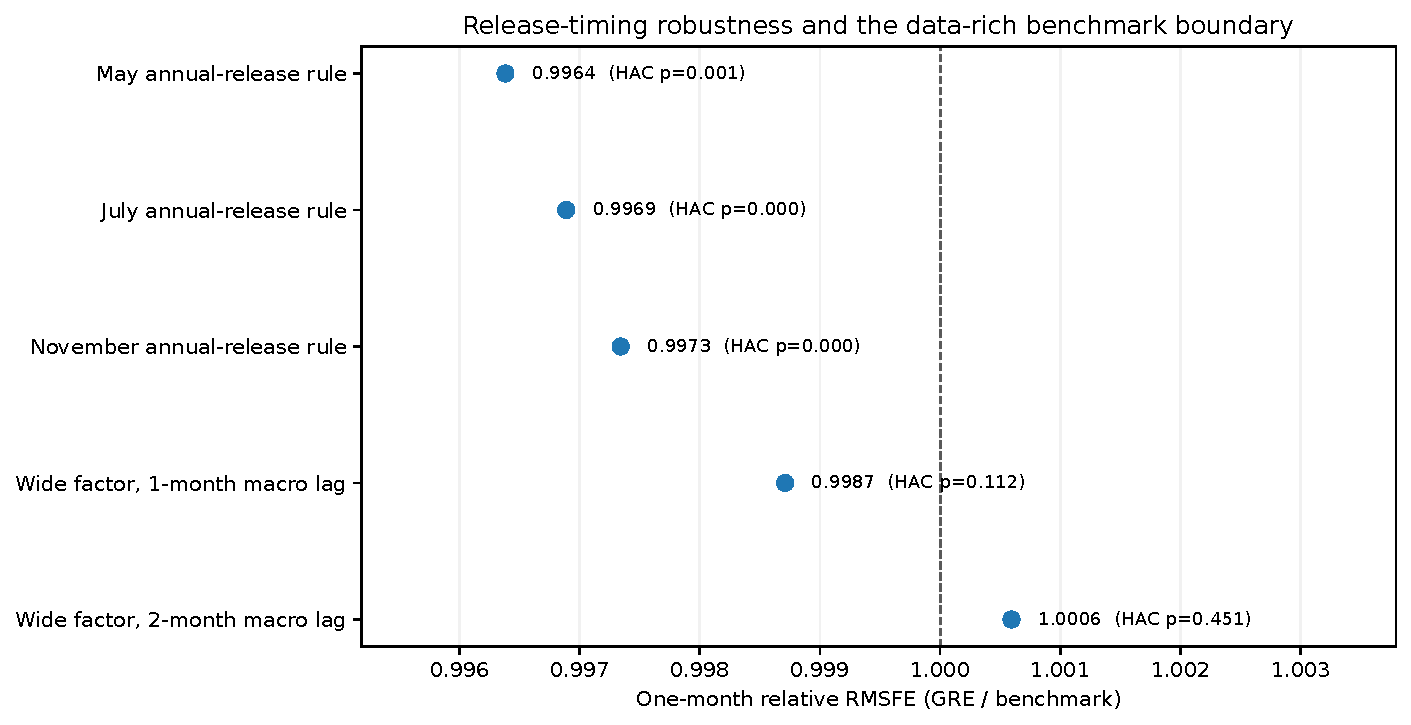
\includegraphics[width=0.90\textwidth]{Figure_Release_Benchmark_Boundary.pdf}
\caption{Release-timing robustness and the data-rich benchmark boundary at the one-month horizon.}
\label{fig:release_benchmark}

\FigureNote{The first three estimates use the same parsimonious country-fixed-effects GDP autoregression with annual benchmark eligibility beginning in May, July, or November of the following year. The final two use six principal components from 159 pre-evaluation-calibrated macro series, lagged one or two months. Parentheses show target-month HAC Clark--West $p$-values; these adjusted-loss tests are distinct from the plotted raw relative RMSFE. The macroeconomic inputs are not archived real-time vintages.}
\end{figure}

\FloatBarrier

\section{Conclusion}\label{sec:conclusion}

The forecasting value of a news-based economic risk measure depends not only on its construction but also on the information used to form the macroeconomic outcome and the historical regressors. We examine that problem with a fixed Growth/Real Economy news score and GDP series constructed from annual benchmarks. The GRE measure combines the prevalence, severity, and prominence of real-economy risk language in newspaper reporting. It is constructed independently of the GDP forecast comparison and remains unchanged across the information-set designs.

The analytical result identifies a property of additive first-difference Denton that is directly relevant to this comparison. An annual benchmark affects monthly levels outside its own year; in the bounded infinite-block solution, off-diagonal coefficients follow an alternating geometric tail with ratio $\mu\simeq-0.264745$. Finite-sample boundaries modify those coefficients. The result describes the propagation of annual-level information through the disaggregation operator, not an inherent direction of forecasting bias. Its practical implication is that using final-vintage reconstructed GDP as a historical regressor may introduce benchmarks unavailable at the time of the forecast.

The African application keeps the GRE predictor, models, countries, and scoring outcomes fixed while changing the information permitted in the historical GDP regressors and the timing of training-label entry. GRE's twelve-month relative RMSFE changes from 0.9961 under retrospective GDP histories to 1.0048 under the publication-lagged rule. The corresponding one-month ratio is 0.9964. That short-horizon advantage is modest, does not hold uniformly across economies, and becomes less persuasive with two-way covariance and a wider factor benchmark. The forecast comparison therefore establishes sensitivity to GDP information treatment, rather than a general predictive advantage for the news index.

The exercise also stops short of a fully historical-vintage design. Annual benchmark values come from a final file and the training targets admitted after the assumed release date remain final-vintage Denton constructions. Actual historical annual releases, country-specific calendars, and training outcomes reconstructed from information available at each origin would be needed for a complete real-time evaluation. The present results nevertheless show that choices made in constructing GDP histories can alter the estimated incremental value of an otherwise unchanged newspaper-based predictor. Researchers using constructed high-frequency macroeconomic series should make those choices part of the forecast-evaluation design rather than treat the final disaggregated history as an observed real-time series.

\section*{Acknowledgments}
None.

\paragraph{Funding} This research did not receive any specific grant from funding agencies in the public, commercial, or not-for-profit sectors.

\section*{Conflict of Interest}
The authors declare that they have no known competing financial interests or personal relationships that could have appeared to influence the work reported in this paper.

\section*{Data Availability Statement}
The data and replication materials that support the findings of this study are available from the corresponding author upon reasonable request. The full underlying news-article archive cannot be redistributed because it contains third-party copyrighted material. The source registry, derived country-month indicators, scoring documentation, code, constructed GDP series, and forecast-evaluation outputs can be provided on request.

\begingroup
\normalsize
\setlength{\bibsep}{0pt plus 0.2ex}
\begin{thebibliography}{99}

\bibitem[Abeyie(2026)]{abeyie2026}
Abeyie, G. A. (2026). Beyond news headlines and TF-IDF: Enhancing text-based
forecasting models with validated collocations and improved attention.
\emph{International Journal of Forecasting, 42}, 752--773.
\url{https://doi.org/10.1016/j.ijforecast.2025.09.002}

\bibitem[Ad{\"a}mmer et al.(2025)]{adaemmer2025}
Ad{\"a}mmer, P., Pr{\"u}ser, J., \& Sch{\"u}ssler, R. A. (2025). Forecasting
macroeconomic tail risk in real time: Do textual data add value?
\emph{International Journal of Forecasting, 41}, 307--320.
\url{https://doi.org/10.1016/j.ijforecast.2024.05.007}

\bibitem[Ahir et al.(2022)]{ahir2022}
Ahir, H., Bloom, N., \& Furceri, D. (2022). The World Uncertainty Index.
NBER Working Paper 29763. \url{https://doi.org/10.3386/w29763}

\bibitem[Akgun et al.(2024)]{akgun2024}
Akgun, O., Pirotte, A., Urga, G., \& Yang, Z. (2024). Equal predictive ability
tests based on panel data with applications to OECD and IMF forecasts.
\emph{International Journal of Forecasting, 40}, 202--228.
\url{https://doi.org/10.1016/j.ijforecast.2023.02.001}

\bibitem[Ardia and Bluteau(2026)]{ardia2026}
Ardia, D., \& Bluteau, K. (2026). Optimal text-based time-series indices.
\emph{International Journal of Forecasting, 42}, 44--60.
\url{https://doi.org/10.1016/j.ijforecast.2025.07.003}

\bibitem[Bae(2024)]{bae2024}
Bae, J. (2024). Factor-augmented forecasting in big data.
\emph{International Journal of Forecasting, 40}, 1660--1688.
\url{https://doi.org/10.1016/j.ijforecast.2024.02.004}

\bibitem[Baker et al.(2016)]{baker2016}
Baker, S. R., Bloom, N., \& Davis, S. J. (2016). Measuring economic policy
uncertainty. \emph{The Quarterly Journal of Economics, 131}, 1593--1636.
\url{https://doi.org/10.1093/qje/qjw024}

\bibitem[Ba{\'n}bura et al.(2013)]{banbura2013}
Ba{\'n}bura, M., Giannone, D., Modugno, M., \& Reichlin, L. (2013).
Now-casting and the real-time data flow. In G. Elliott \& A. Timmermann
(Eds.), \emph{Handbook of Economic Forecasting} (Vol. 2A, pp. 195--237).
Elsevier. \url{https://doi.org/10.1016/B978-0-444-53683-9.00004-9}

\bibitem[Bok et al.(2018)]{bok2018}
Bok, B., Caratelli, D., Giannone, D., Sbordone, A. M., \& Tambalotti, A.
(2018). Macroeconomic nowcasting and forecasting with big data. \emph{Annual
Review of Economics, 10}, 615--643.
\url{https://doi.org/10.1146/annurev-economics-080217-053214}

\bibitem[Caldara and Iacoviello(2022)]{caldara2022}
Caldara, D., \& Iacoviello, M. (2022). Measuring geopolitical risk.
\emph{American Economic Review, 112}, 1194--1225.
\url{https://doi.org/10.1257/aer.20191823}

\bibitem[Chow and Lin(1971)]{chowlin1971}
Chow, G. C., \& Lin, A. (1971). Best linear unbiased interpolation, distribution, and extrapolation of time series by related series.
\emph{The Review of Economics and Statistics, 53}(4), 372--375.
\url{https://doi.org/10.2307/1928739}

\bibitem[Clark and West(2007)]{clarkwest2007}
Clark, T. E., \& West, K. D. (2007). Approximately normal tests for equal
predictive accuracy in nested models. \emph{Journal of Econometrics, 138},
291--311. \url{https://doi.org/10.1016/j.jeconom.2006.05.023}

\bibitem[Coroneo and Iacone(2025)]{coroneo2025}
Coroneo, L., \& Iacone, F. (2025). Testing for equal predictive accuracy with
strong dependence. \emph{International Journal of Forecasting, 41},
1073--1092. \url{https://doi.org/10.1016/j.ijforecast.2024.11.003}

\bibitem[Croushore(2006)]{croushore2006}
Croushore, D. (2006). Forecasting with real-time macroeconomic data. In
G. Elliott, C. W. J. Granger, \& A. Timmermann (Eds.), \emph{Handbook of
Economic Forecasting} (Vol. 1, pp. 961--982). Elsevier.
\url{https://doi.org/10.1016/S1574-0706(05)01017-7}

\bibitem[Croushore and Stark(2001)]{croushorestark2001}
Croushore, D., \& Stark, T. (2001). A real-time data set for macroeconomists.
\emph{Journal of Econometrics, 105}, 111--130.
\url{https://doi.org/10.1016/S0304-4076(01)00072-0}

\bibitem[Denton(1971)]{denton1971}
Denton, F. T. (1971). Adjustment of monthly or quarterly series to annual
totals: An approach based on quadratic minimization. \emph{Journal of the
American Statistical Association, 66}, 99--102.
\url{https://doi.org/10.1080/01621459.1971.10482227}

\bibitem[Eilers(2003)]{eilers2003}
Eilers, P. H. C. (2003). A perfect smoother. \emph{Analytical Chemistry, 75},
3631--3636. \url{https://doi.org/10.1021/ac034173t}

\bibitem[Feng(2009)]{feng2009}
Feng, H. (2009). Real-time or current vintage: Does the type of data matter for
forecasting and model selection? \emph{Journal of Forecasting, 28}, 183--193.
\url{https://doi.org/10.1002/for.1089}

\bibitem[Fern\'{a}ndez(1981)]{fernandez1981}
Fern\'{a}ndez, R. B. (1981). A methodological note on the estimation of time series.
\emph{The Review of Economics and Statistics, 63}(3), 471--476.
\url{https://doi.org/10.2307/1924371}

\bibitem[Gentzkow et al.(2019)]{gentzkow2019}
Gentzkow, M., Kelly, B., \& Taddy, M. (2019). Text as data. \emph{Journal of
Economic Literature, 57}, 535--574.
\url{https://doi.org/10.1257/jel.20181020}

\bibitem[Giannone et al.(2008)]{giannone2008}
Giannone, D., Reichlin, L., \& Small, D. (2008). Nowcasting: The real-time
informational content of macroeconomic data. \emph{Journal of Monetary
Economics, 55}, 665--676.
\url{https://doi.org/10.1016/j.jmoneco.2008.05.010}

\bibitem[International Monetary Fund(2017)]{imfqna2017}
International Monetary Fund. (2017). \emph{Quarterly national accounts manual: 2017 edition}. International Monetary Fund.

\bibitem[Kim and Swanson(2018)]{kimswanson2018}
Kim, H. H., \& Swanson, N. R. (2018). Methods for backcasting, nowcasting and forecasting using factor-MIDAS: With an application to Korean GDP.
\emph{Journal of Forecasting, 37}(3), 281--302.
\url{https://doi.org/10.1002/for.2499}

\bibitem[Litterman(1983)]{litterman1983}
Litterman, R. B. (1983). A random walk, Markov model for the distribution of time series.
\emph{Journal of Business \& Economic Statistics, 1}(2), 169--173.
\url{https://doi.org/10.1080/07350015.1983.10509336}

\bibitem[Pfarrhofer(2024)]{pfarrhofer2024}
Pfarrhofer, M. (2024). Forecasts with Bayesian vector autoregressions under real time conditions.
\emph{Journal of Forecasting, 43}(3), 771--801.
\url{https://doi.org/10.1002/for.3055}

\bibitem[Qu et al.(2024)]{qu2024}
Qu, R., Timmermann, A., \& Zhu, Y. (2024). Comparing forecasting performance
with panel data. \emph{International Journal of Forecasting, 40}, 918--941.
\url{https://doi.org/10.1016/j.ijforecast.2023.08.001}

\bibitem[R{\"u}nstler et al.(2009)]{ruenstler2009}
R{\"u}nstler, G., Barhoumi, K., Benk, S., Cristadoro, R., Den Reijer, A.,
Jakaitiene, A., Jelonek, P., Rua, A., Ruth, K., \& Van Nieuwenhuyze, C. (2009).
Short-term forecasting of GDP using large datasets: A pseudo real-time forecast
evaluation exercise. \emph{Journal of Forecasting, 28}, 595--611.
\url{https://doi.org/10.1002/for.1105}

\bibitem[Seo(2025)]{seo2025}
Seo, B. (2025). Econometric forecasting using ubiquitous news text:
Text-enhanced factor model. \emph{International Journal of Forecasting, 41},
1055--1072. \url{https://doi.org/10.1016/j.ijforecast.2024.11.001}

\bibitem[Stock and Watson(2002)]{stockwatson2002}
Stock, J. H., \& Watson, M. W. (2002). Macroeconomic forecasting using
diffusion indexes. \emph{Journal of Business \& Economic Statistics, 20},
147--162. \url{https://doi.org/10.1198/073500102317351921}

\bibitem[Stock and Watson(2004)]{stockwatson2004}
Stock, J. H., \& Watson, M. W. (2004). Combination forecasts of output growth
in a seven-country data set. \emph{Journal of Forecasting, 23}, 405--430.
\url{https://doi.org/10.1002/for.928}

\bibitem[Timmermann(2006)]{timmermann2006}
Timmermann, A. (2006). Forecast combinations. In G. Elliott,
C. W. J. Granger, \& A. Timmermann (Eds.), \emph{Handbook of Economic
Forecasting} (Vol. 1, pp. 135--196). Elsevier.
\url{https://doi.org/10.1016/S1574-0706(05)01004-9}

\bibitem[Zheng et al.(2024)]{zheng2024}
Zheng, T., Fan, X., Jin, W., \& Fang, K. (2024). Words or numbers?
Macroeconomic nowcasting with textual and macroeconomic data.
\emph{International Journal of Forecasting, 40}, 746--761.
\url{https://doi.org/10.1016/j.ijforecast.2023.05.006}

\end{thebibliography}
\endgroup


\end{document}
